\section{Программная реализация}

В рамках курсовой работы был разработан прототип программного обеспечения, рассчитывающего электродинамические структуры методом конечных разностей во временной области с использованием графического процессора. Применение ГПУ было призвано улучшить производительность вычислений.

\subsection{Программная реализация сетки И}

Разработка программы велась на языке С++, поэтому в качестве программного представления сетки И было решено использовать тип данных «класс». Входными аргументами конструктора класса выступают линейные размеры сетки в ячейках и величины $ \Delta{x} $, $ \Delta{y} $, $ \Delta{z} $, $ \Delta{t} $.

Из рис.~\ref{fig:YeeGrid} легко заметить, что все данные сетки (значения диэлектрической и магнитной проницаемости, удельной электрической и магнитной проводимостей, проекций векторов электрической и магнитной напряжённостей поля на координатные оси) представляют собой трёхмерные массивы с номерами ячеек $ i $, $ j $, $ k $ в качестве индексов.

\subsection{Базовый алгоритм FDTD}

Первым этапом создания программной реализации метода конечных разностей во временной области стало выделение из формул базового алгоритма коэффициентов и написание функций для их расчёта. Неизменность коэффициентов позволяет рассчитывать их единожды при старте программы и использовать готовые значения при пересчёте характеристик поля в каждой ячейке в каждый момент времени.

\begin{equation}
\label{eq:CDCoeffs}
    \newcommand\XA{\displaystyle
        \frac{\Delta{t}}{P}}
    \newcommand\XB{\displaystyle
        \frac{\sigma\Delta{t}}{2P}}
    % --
    C = \frac{\XA}{1+\XB}, \quad
    D = \frac{1-\XB}{1+\XB}.
\end{equation}

Данные коэффициенты приведены в формуле~\eqref{eq:CDCoeffs}, где $ P $ --- проницаемость материала (диэлектрическая и магнитная для проекций векторов $\vec{E}$  и $\vec{H}$ соответственно), а $\sigma$ --- удельная проводимость (электрическая и магнитная для проекций векторов $\vec{E}$  и $\vec{H}$ соответственно).

Следующим шагом стало написание функций, предназначенных для расчёта проекций векторов электрической и магнитной напряжённости во всех точках счётного объёма в какой-либо момент времени. Программный код, производящий расчёт компонент вектора магнитной напряжённости, приведён в приложении~А.

\subsection{Тестовая задача}

Симметричный вибратор --- простейшая система для получения электромагнитных колебаний. Представляет собой электрический диполь, дипольный момент которого быстро изменяется во времени, и является развёрнутым колебательным контуром с минимальной ёмкостью и индуктивностью.

В исходном коде конечной программы симметричный вибратор был представлен двадцатью ячейками счётного объёма, расположенными вдоль оси~$ Z $, с отличными от остальных удельной электрической проводимостью материала~$\sigma$
и абсолютной диэлектрической проницаемостью материала~$\varepsilon$. Длина волны была подобрана таким образом, чтобы отношение длины диполя к длине волны было равно двум.

\subsection{Реализация резистивного источника}

Следующим этапом моделирования резистивного источника стал пересчёт
значений проекции вектора $ \vec{E} $ на ось~$ Z $. Во избежание проверки каждой ячейки на наличие там проводящих структур было принято решение сохранять информацию обо всех ячейках до расчёта значений вектора электрической напряжённости, затем выполнять этот расчёт и, наконец, пересчёт значений проекции
вектора~$ \vec{E} $ на ось~$ Z $ только в точках присутствия элементов источника.

\begin{figure}[p]
    \centering
    \vspace{30mm}
    \begin{subfigure}[b]{0.3\textwidth}
        
\includegraphics[width=\textwidth]{include/graphics/image6}

        \label{fieldFig:1st}
    \end{subfigure}
    ~ %add desired spacing between images, e. g. ~, \quad, \qquad, \hfill etc. 
      %(or a blank line to force the subfigure onto a new line)
    \begin{subfigure}[b]{0.3\textwidth}
        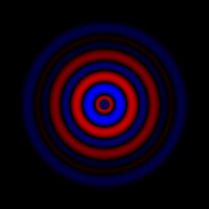
\includegraphics[width=\textwidth]{include/graphics/image7}
  
        \label{fieldFig:2nd}
    \end{subfigure}
    ~ %add desired spacing between images, e. g. ~, \quad, \qquad, \hfill etc. 
    %(or a blank line to force the subfigure onto a new line)
    \begin{subfigure}[b]{0.3\textwidth}
        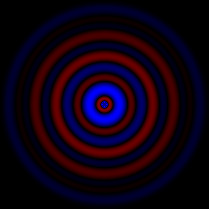
\includegraphics[width=\textwidth]{include/graphics/image8}

        \label{fieldFig:3rd}
    \end{subfigure}
    
\bigskip
        \begin{subfigure}[b]{0.3\textwidth}
        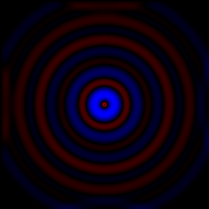
\includegraphics[width=\textwidth]{include/graphics/image9}

        \label{fieldFig:4th}
    \end{subfigure}
    ~ %add desired spacing between images, e. g. ~, \quad, \qquad, \hfill etc. 
      %(or a blank line to force the subfigure onto a new line)
    \begin{subfigure}[b]{0.3\textwidth}
        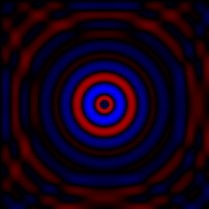
\includegraphics[width=\textwidth]{include/graphics/image10}
  
        \label{fieldFig:5th}
    \end{subfigure}
    ~ %add desired spacing between images, e. g. ~, \quad, \qquad, \hfill etc. 
    %(or a blank line to force the subfigure onto a new line)
    \begin{subfigure}[b]{0.3\textwidth}
        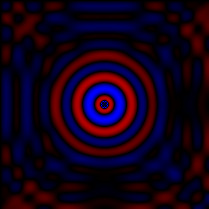
\includegraphics[width=\textwidth]{include/graphics/image11}

        \label{fieldFig:6th}
    \end{subfigure}

    \caption{Изменение электрического поля во времени (вид сверху)}\label{fig:animals}
\end{figure}

\subsection{Перенос вычислительной нагрузки на графический процессор}

В целях увеличения производительности функции расчёта значений про-
екций векторов электрической и магнитной напряжённостей были изменены
для исполнения на графических процессорах. Из двух технологий, позволяю-
щих осуществить расчёт на GPU: NVIDIA CUDA и OpenCL --- была выбрана
вторая, так как она поддерживает процессоры не только производства компа-
нии NVIDIA, но и AMD.

Для облегчения работы с фреймворком OpenCL была использована библиотека EasyCL. Код расчёта компонент вектора магнитной напряжённости
приведён в приложении~Б.

\begin{figure}[p]
\centering
\captionsetup{justification=centering}
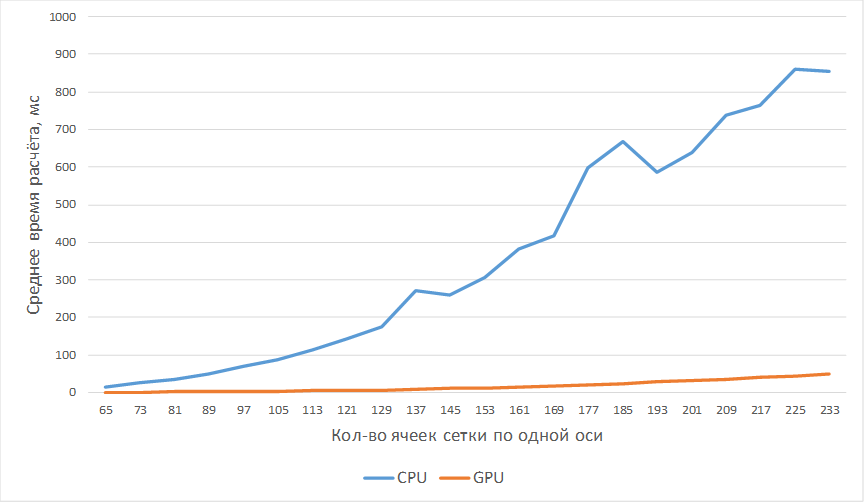
\includegraphics[width=0.95\textwidth]{include/graphics/image12}
\caption{Зависимость среднего времени расчёта компонент вектора $\vec{H}$ в конкретный момент времени во всех ячейках от размеров сетки}
\label{fig:1stComparsion}
\end{figure}
\begin{figure}[p]
\centering
\captionsetup{justification=centering}
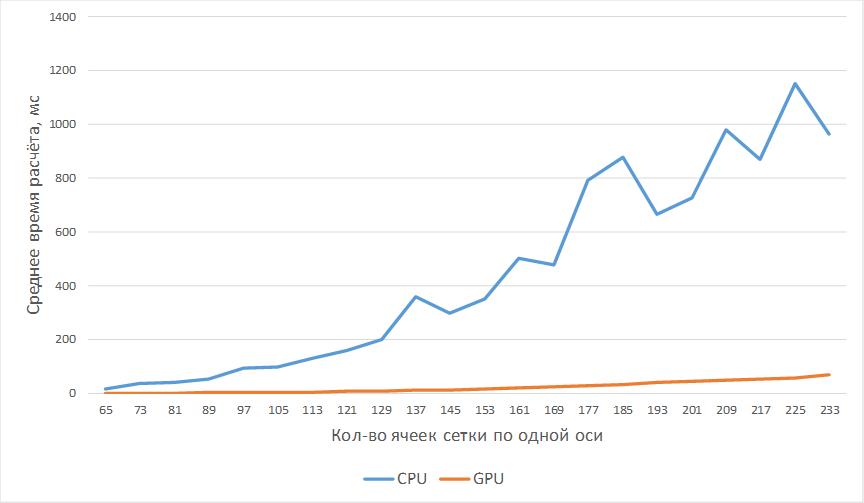
\includegraphics[width=0.95\textwidth]{include/graphics/image13}
\caption{Зависимость среднего времени расчёта компонент вектора $\vec{E}$ в конкретный момент времени во всех ячейках от размеров сетки}
\label{fig:2ndComparsion}
\end{figure}


\clearpage